% Proposed-framework diagram for the mid-evaluation poster (Phase 3). Build:
%   cd report/figures && ~/.local/bin/tectonic -X compile poster_framework.tex
%   pdftoppm -png -r 300 -singlefile poster_framework.pdf poster_framework
\documentclass[border=6pt,12pt]{standalone}
\usepackage{fontspec}\setmainfont{Noto Sans}\hyphenpenalty=10000\exhyphenpenalty=10000
\usepackage{tikz}\usetikzlibrary{arrows.meta,fit,backgrounds,positioning}
\definecolor{cIn}{HTML}{E7EEF7}\definecolor{cEv}{HTML}{D6EAF8}\definecolor{cMod}{HTML}{CFE2F3}
\definecolor{cSt}{HTML}{1F5F99}\definecolor{cOrg}{HTML}{D9EAD3}\definecolor{cMan}{HTML}{FCE5CD}\definecolor{cSyn}{HTML}{F4CCCC}
\definecolor{cLine}{HTML}{2E4A66}
\begin{document}
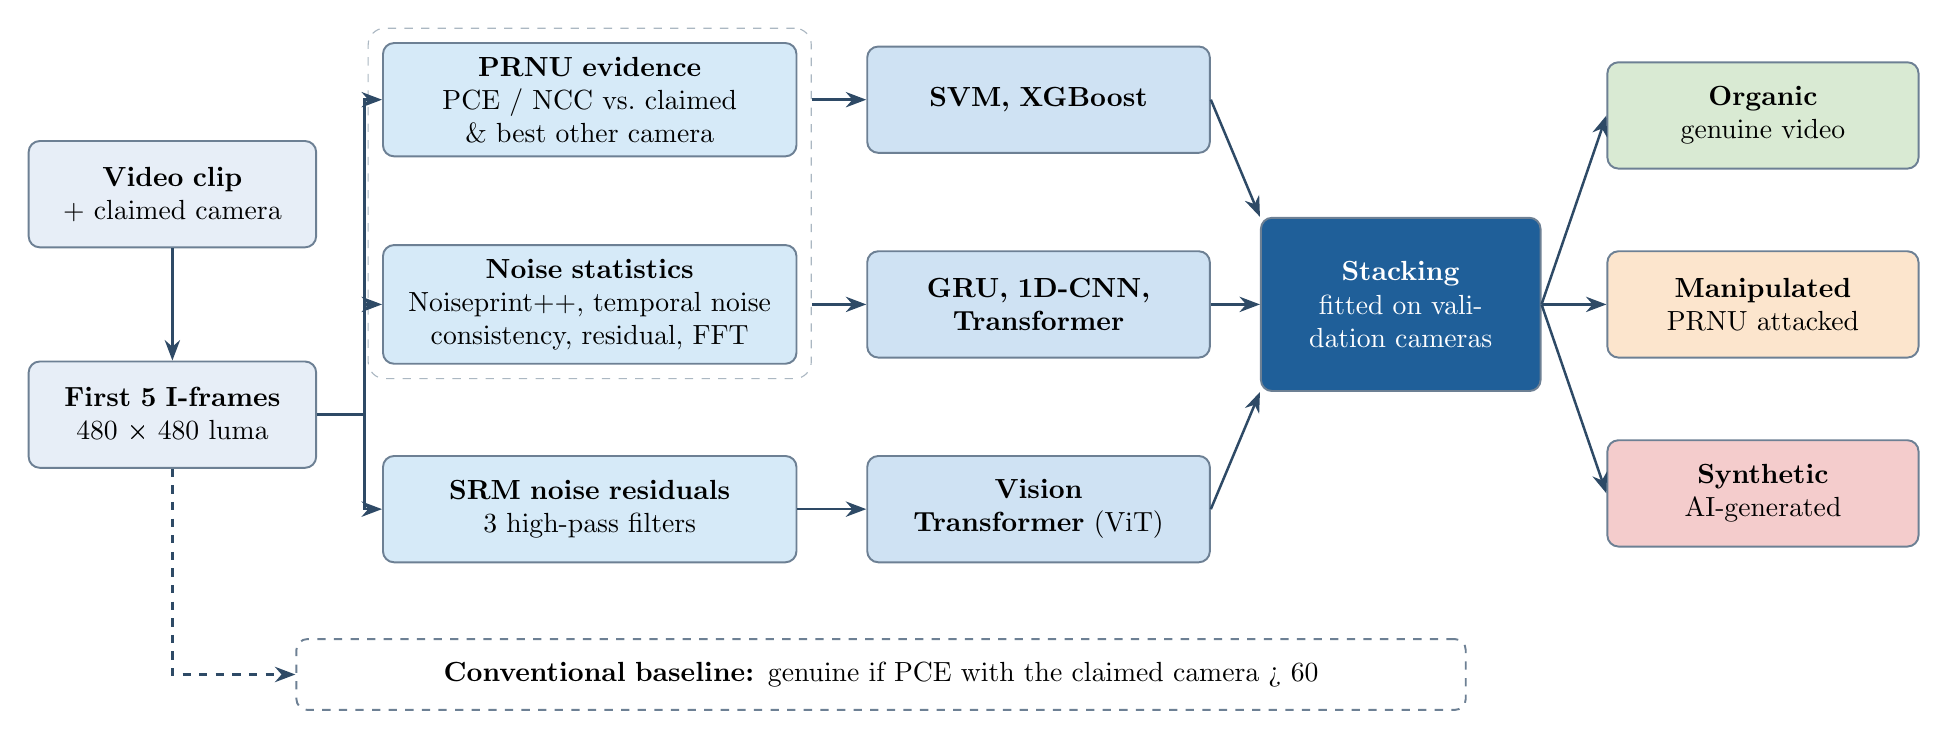
\begin{tikzpicture}[>={Stealth[length=2.6mm]},
  box/.style={draw=cLine!70, rounded corners=4pt, align=center, line width=0.7pt, inner sep=5pt, minimum height=1.35cm},
  arr/.style={->, draw=cLine, line width=0.9pt}]
\node[box, fill=cIn, text width=3.3cm] (in) at (0,1.4) {\textbf{Video clip}\\+ claimed camera};
\node[box, fill=cIn, text width=3.3cm] (fr) at (0,-1.4) {\textbf{First 5 I-frames}\\480 × 480 luma};
\node[box, fill=cEv, text width=4.9cm] (e1) at (5.3,2.6) {\textbf{PRNU evidence}\\PCE / NCC vs.\ claimed \& best other camera};
\node[box, fill=cEv, text width=4.9cm] (e2) at (5.3,0) {\textbf{Noise statistics}\\Noiseprint++, temporal noise consistency, residual, FFT};
\node[box, fill=cEv, text width=4.9cm] (e3) at (5.3,-2.6) {\textbf{SRM noise residuals}\\3 high-pass filters};
\node[box, fill=cMod, text width=4.0cm] (m1) at (11.0,2.6) {\textbf{SVM, XGBoost}};
\node[box, fill=cMod, text width=4.0cm] (m2) at (11.0,0) {\textbf{GRU, 1D-CNN,}\\\textbf{Transformer}};
\node[box, fill=cMod, text width=4.0cm] (m3) at (11.0,-2.6) {\textbf{Vision}\\\textbf{Transformer} (ViT)};
\node[box, fill=cSt, text=white, text width=3.2cm, minimum height=2.2cm] (st) at (15.6,0) {\textbf{Stacking}\\fitted on validation cameras};
\node[box, fill=cOrg, text width=3.6cm] (o1) at (20.2,2.4) {\textbf{Organic}\\genuine video};
\node[box, fill=cMan, text width=3.6cm] (o2) at (20.2,0) {\textbf{Manipulated}\\PRNU attacked};
\node[box, fill=cSyn, text width=3.6cm] (o3) at (20.2,-2.4) {\textbf{Synthetic}\\AI-generated};
\node[box, dashed, fill=white, text width=14.5cm, minimum height=0.9cm] (bl) at (9.0,-4.7)
  {\textbf{Conventional baseline:} genuine if PCE with the claimed camera > 60};
\begin{scope}[on background layer]
  \node[draw=cLine!40, dashed, rounded corners=6pt, fit=(e1)(e2), inner sep=5pt] (feat) {};
\end{scope}
\draw[arr] (in) -- (fr);
\draw[arr] (fr.east) -- ++(0.6,0) |- (e1.west);
\draw[arr] (fr.east) -- ++(0.6,0) |- (e2.west);
\draw[arr] (fr.east) -- ++(0.6,0) |- (e3.west);
\draw[arr] (feat.east |- m1) -- (m1); \draw[arr] (feat.east |- m2) -- (m2); \draw[arr] (e3) -- (m3);
\draw[arr] (m1.east) -- (st.north west); \draw[arr] (m2) -- (st); \draw[arr] (m3.east) -- (st.south west);
\draw[arr] (st.east) -- (o1.west); \draw[arr] (st) -- (o2); \draw[arr] (st.east) -- (o3.west);
\draw[arr, dashed] (fr.south) |- (bl.west);
\end{tikzpicture}
\end{document}
